\section{Interfejs użytkownika (Zofia Sosińska)}\label{chap:ui}
Projekt interfejsu użytkownika przewiduje tryb podstawowy z zawsze widocznymi elementami oraz dynamicznie pojawiające okna, wywoływane za pomocą konkretnych klawiszy. 
 Zadaniem każdej składowej nich będzie odzwierciedlenie pewnego skrawka aktualnego stanu wiedzy granej postaci z naciskiem na najpotrzebniejsze w danej chwili informacje. Przewidziane są:
 \begin{itemize}
    \item menu stawiania budynków; 
    \item menu wydawania komend;
    \item menu zapisu;
    \item informacja o możliwej interakcji;
    \item dziennik z zadaniami;
    \item ekran końca gry.
\end{itemize}
	
\subsection{Interfejs podstawowy}
Interfejs podstawowy przewiduje funkcje, takie jak pokazanie:
\begin{itemize}
    \item aktualnego czasu w grze, aby stworzyć iluzję upływającego czasu w świecie gry; 
    \item surowców i funduszy, aby nie był obarczony kalkulacjami przy każdym zakupie lub przypływie zasobów
    \item kompasu, aby ułatwić nawigację;
    \item stan zdrowia gracza, aby zasygnalizować mu, czy przypadkiem nie rozsądniejsze będzie wycofanie się z potyczki;
    \item etap, na którym są przypisane graczowi zadania, aby przypomnieć mu, że na takowe się zgodził.
\end{itemize}
Inspiracją dla górnego paska z informacjami jest ten użyty w grze Warcraft 3 (por.\ref{c:pasek_war3}). Prostota i surowość stylu będą współgrać z klimatem gry.

W naszej grze skupimy się jednak na tym, aby interfejs użytkownika zabierał jak najmniej miejsca. Dlatego też projekt zakłada, że poszczególne obiekty nie będą ze sobą połączone, a jedynie “dryfować” w przestrzeni.
Jako ważny element tej części UI zawarty zostanie kompas, wzorowany na tym z gry The Elder Scrolls V: Skyrim (por.\ref{chap:skrm}).
\begin{figure}[htbp]
    \centering
    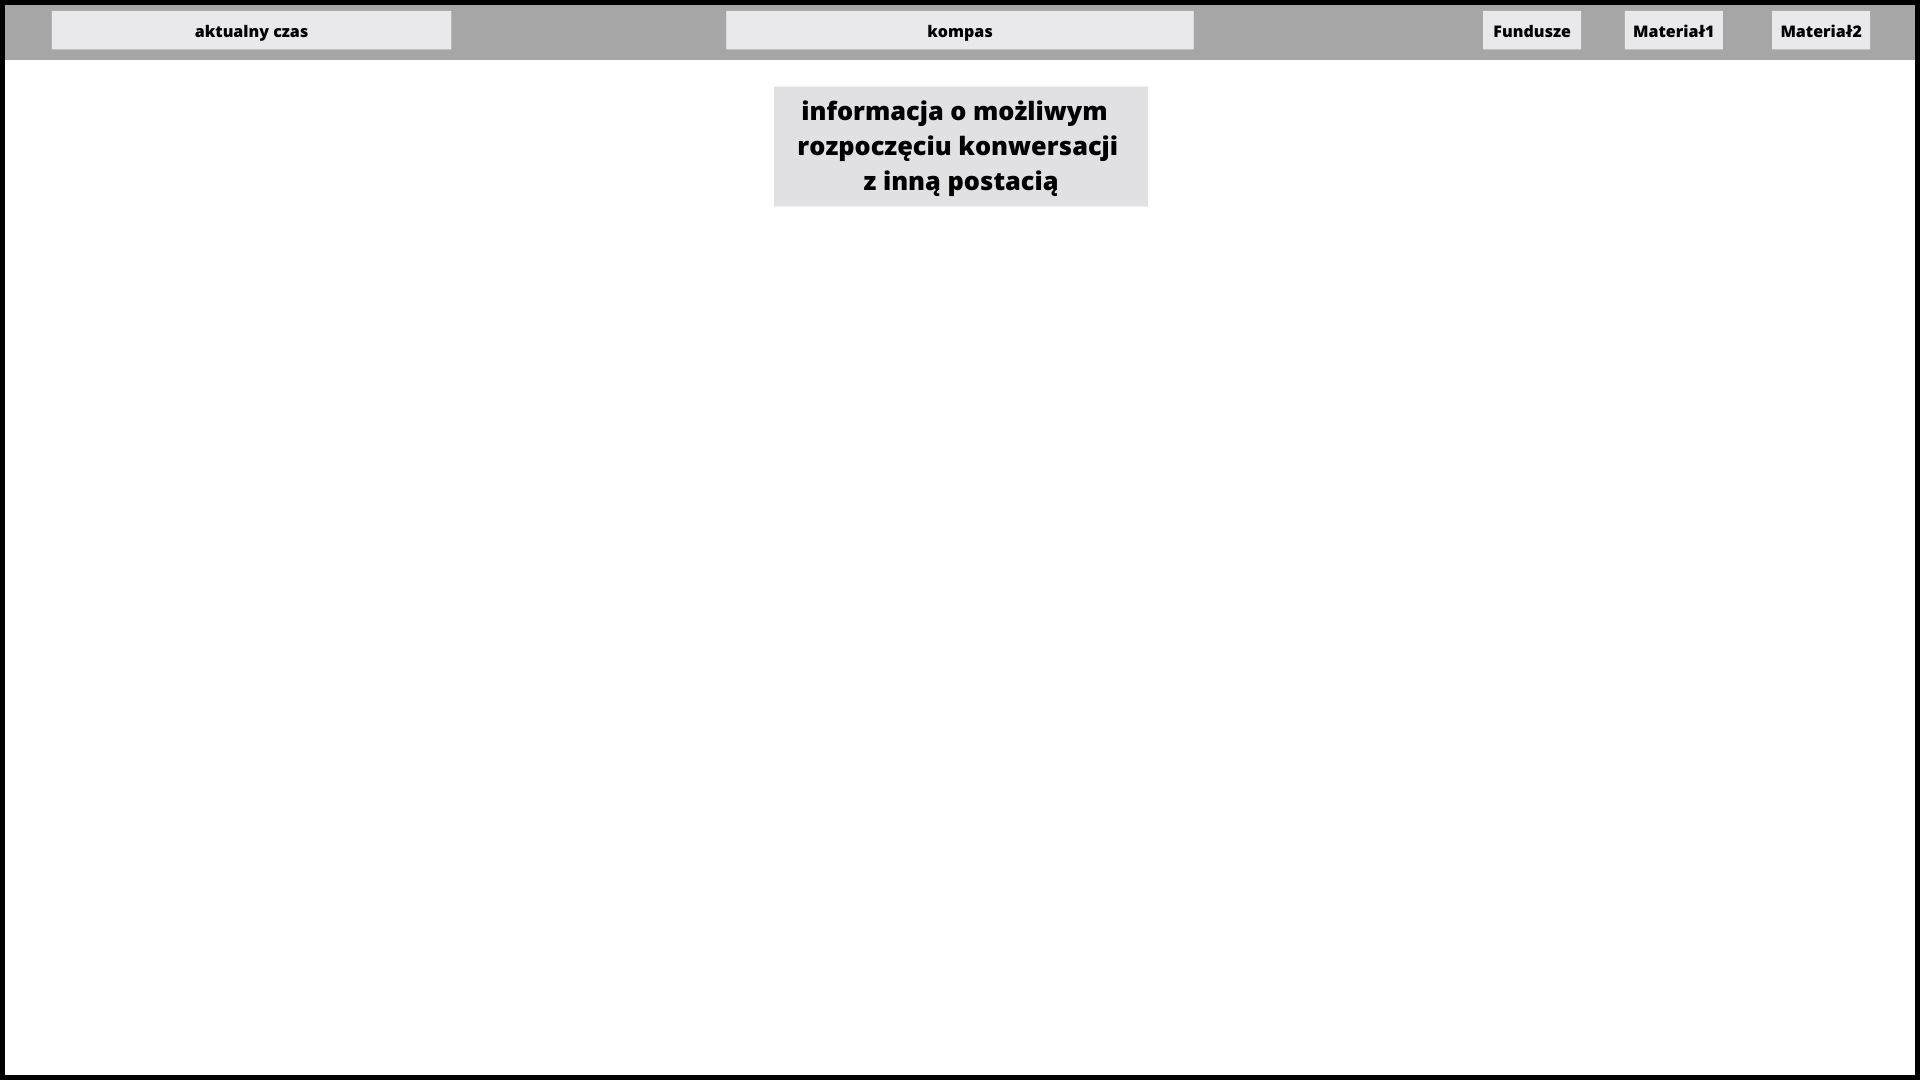
\includegraphics[width=0.9\textwidth]{images/ui/ui_proj_ogolne.jpg}
    \caption{Projekt interfejsu podstawowego UI.
    }\label{fig:ui_main}
\end{figure}
 
\subsection{Menu stawiania budynków}
 W menu stawiania budynków informacje wcześniej przedstawione zostaną na ekranie. Dodatkowo pokażą nam się dostępne do zbudowania budynki, a po wybraniu pojawią się przed nami. Po zatwierdzeniu budynek zostanie wybudowany.
	Inspiracją do przedstawienia dostępnych budowli jest rozwiązanie gry Orcs must die! (por. \ref{chap:omd}).
\begin{figure}[htbp]
    \centering
    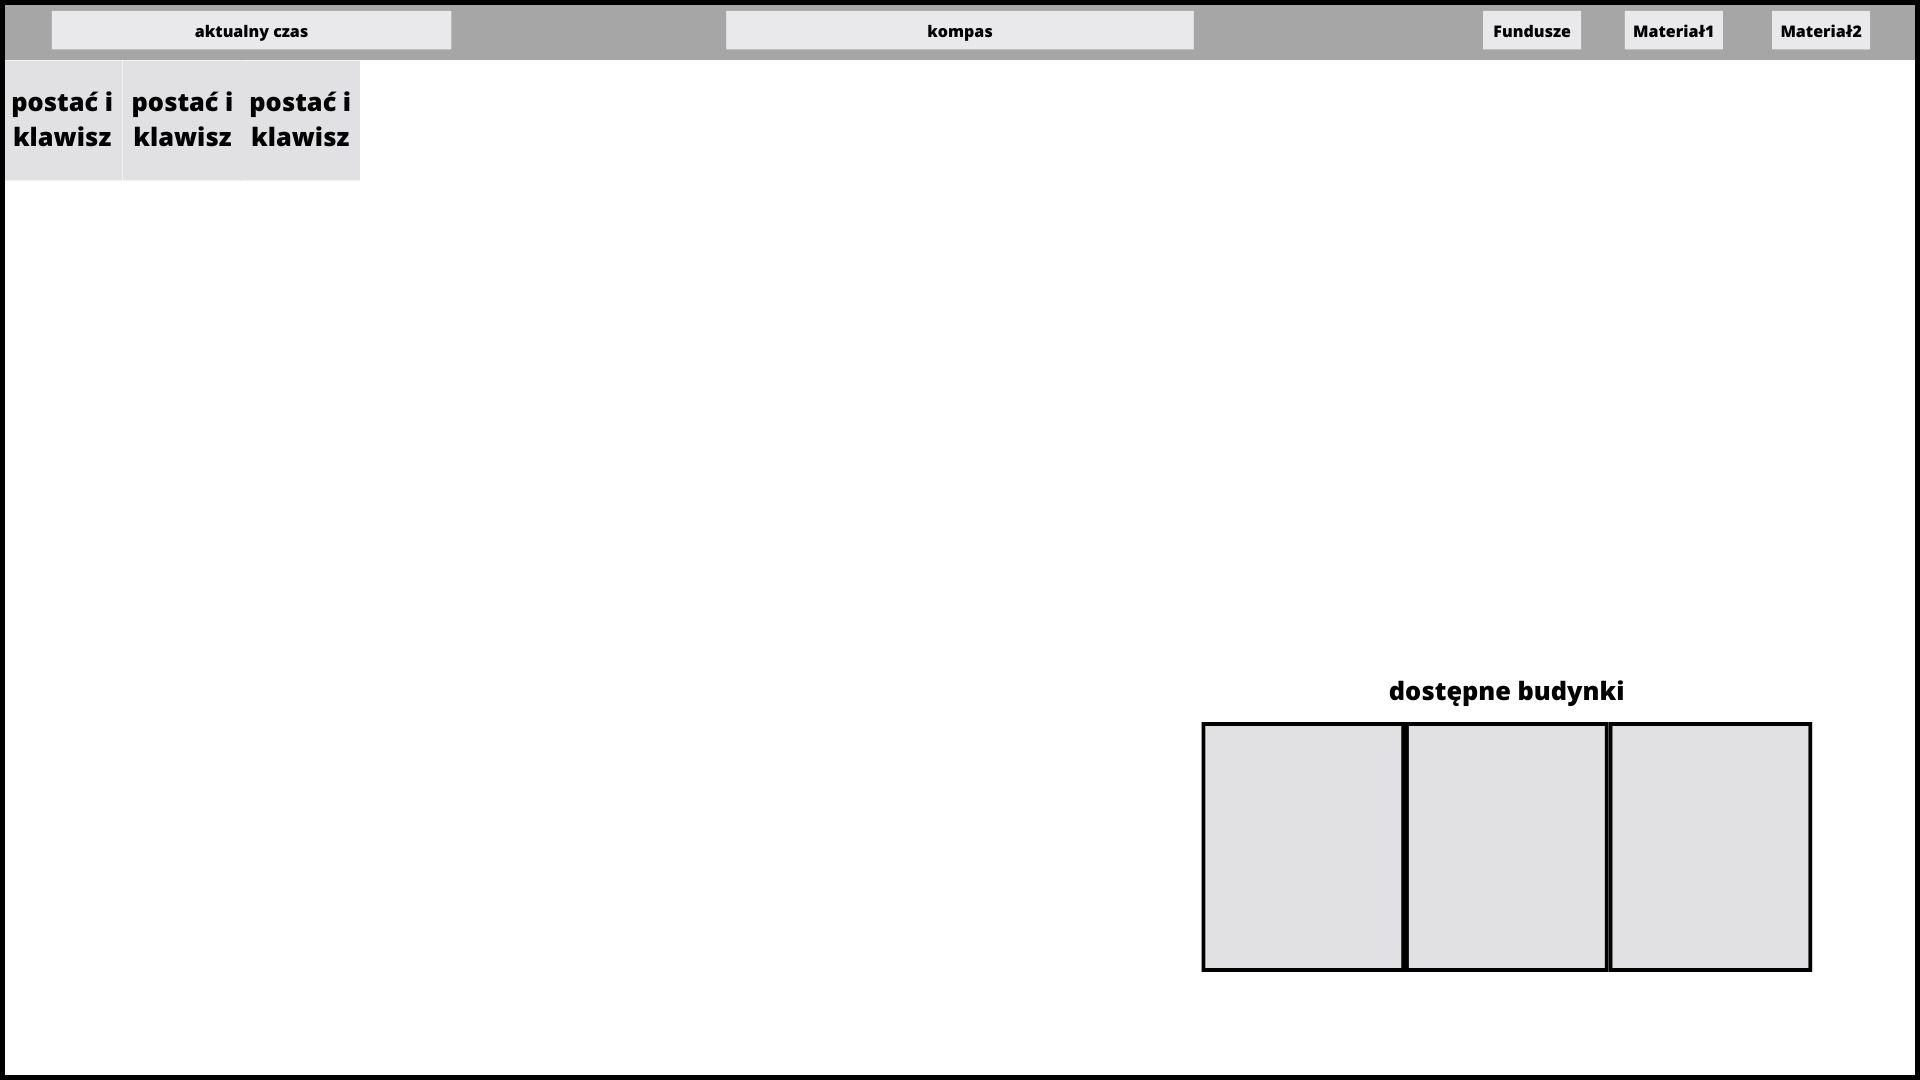
\includegraphics[width=0.9\textwidth]{images/ui/ui_proj_budowanie.jpg}
    \caption{Projekt menu stawiania budynków.
    }\label{fig:ui_bud}
\end{figure}

\subsection{Menu wydawania komend}
Po zdobyciu towarzyszów walki kluczowe jest udostępnienie mechaniki sterowania nimi. Będzie to zrealizowane za pomocą menu wydawania komend.
Projekt przewiduje zrobić to za pomocą wyświtlenia listy dostępnych komend i klawiszy, po których naciśnięciu zostanie konkretna wybrana.
\begin{figure}[htbp]
    \centering
    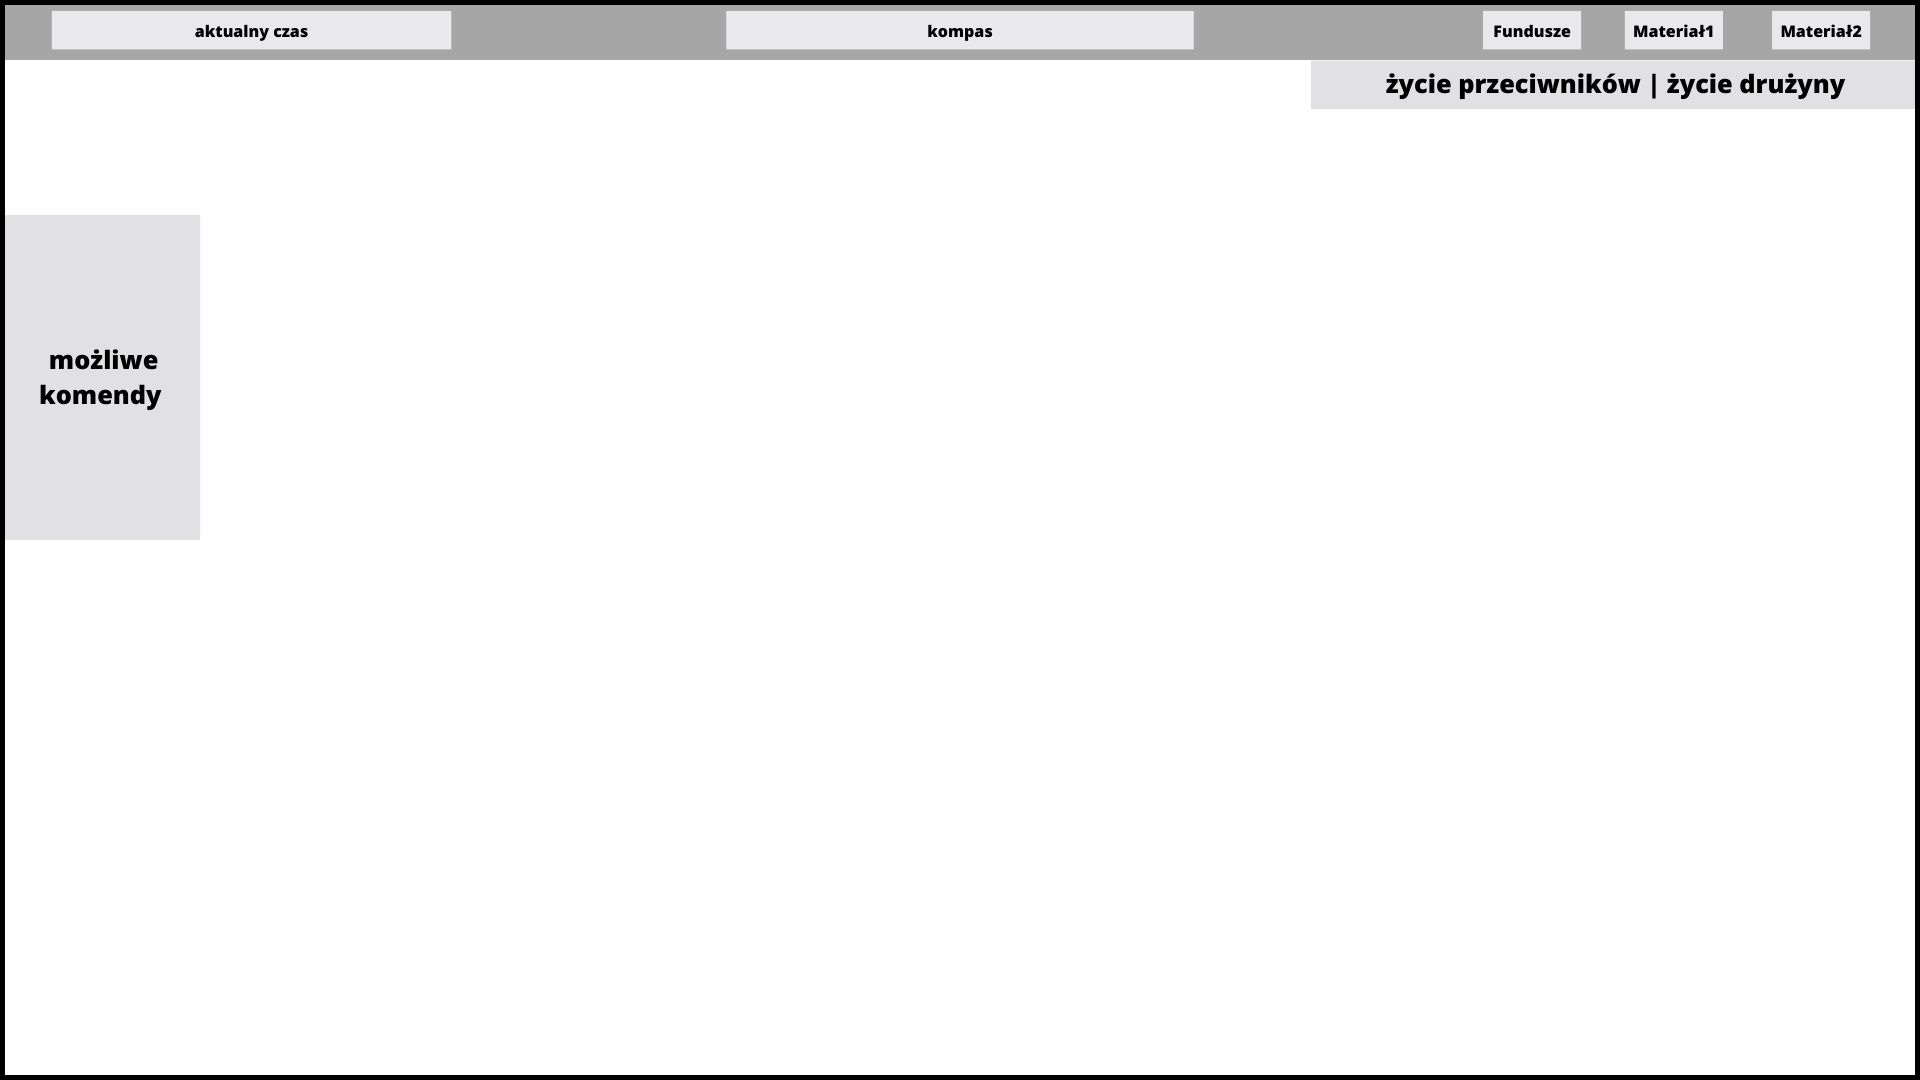
\includegraphics[width=0.9\textwidth]{images/ui/ui_proj_walka.jpg}
    \caption{Projekt menu wydawania komend.}\label{fig:cmd_menu}
\end{figure}

\subsection{Menu zapisu}
Aby umożliwić zapis gry przygotowane zostanie specjalne dla tego zadania menu, wyświetlane na środku ekranu. Najważniejszą informacją 
wyświetlaną na nim będzie nazwa pliku, aby gracz mógł później go odnaleźć.
\begin{figure}[htbp]
    \centering
    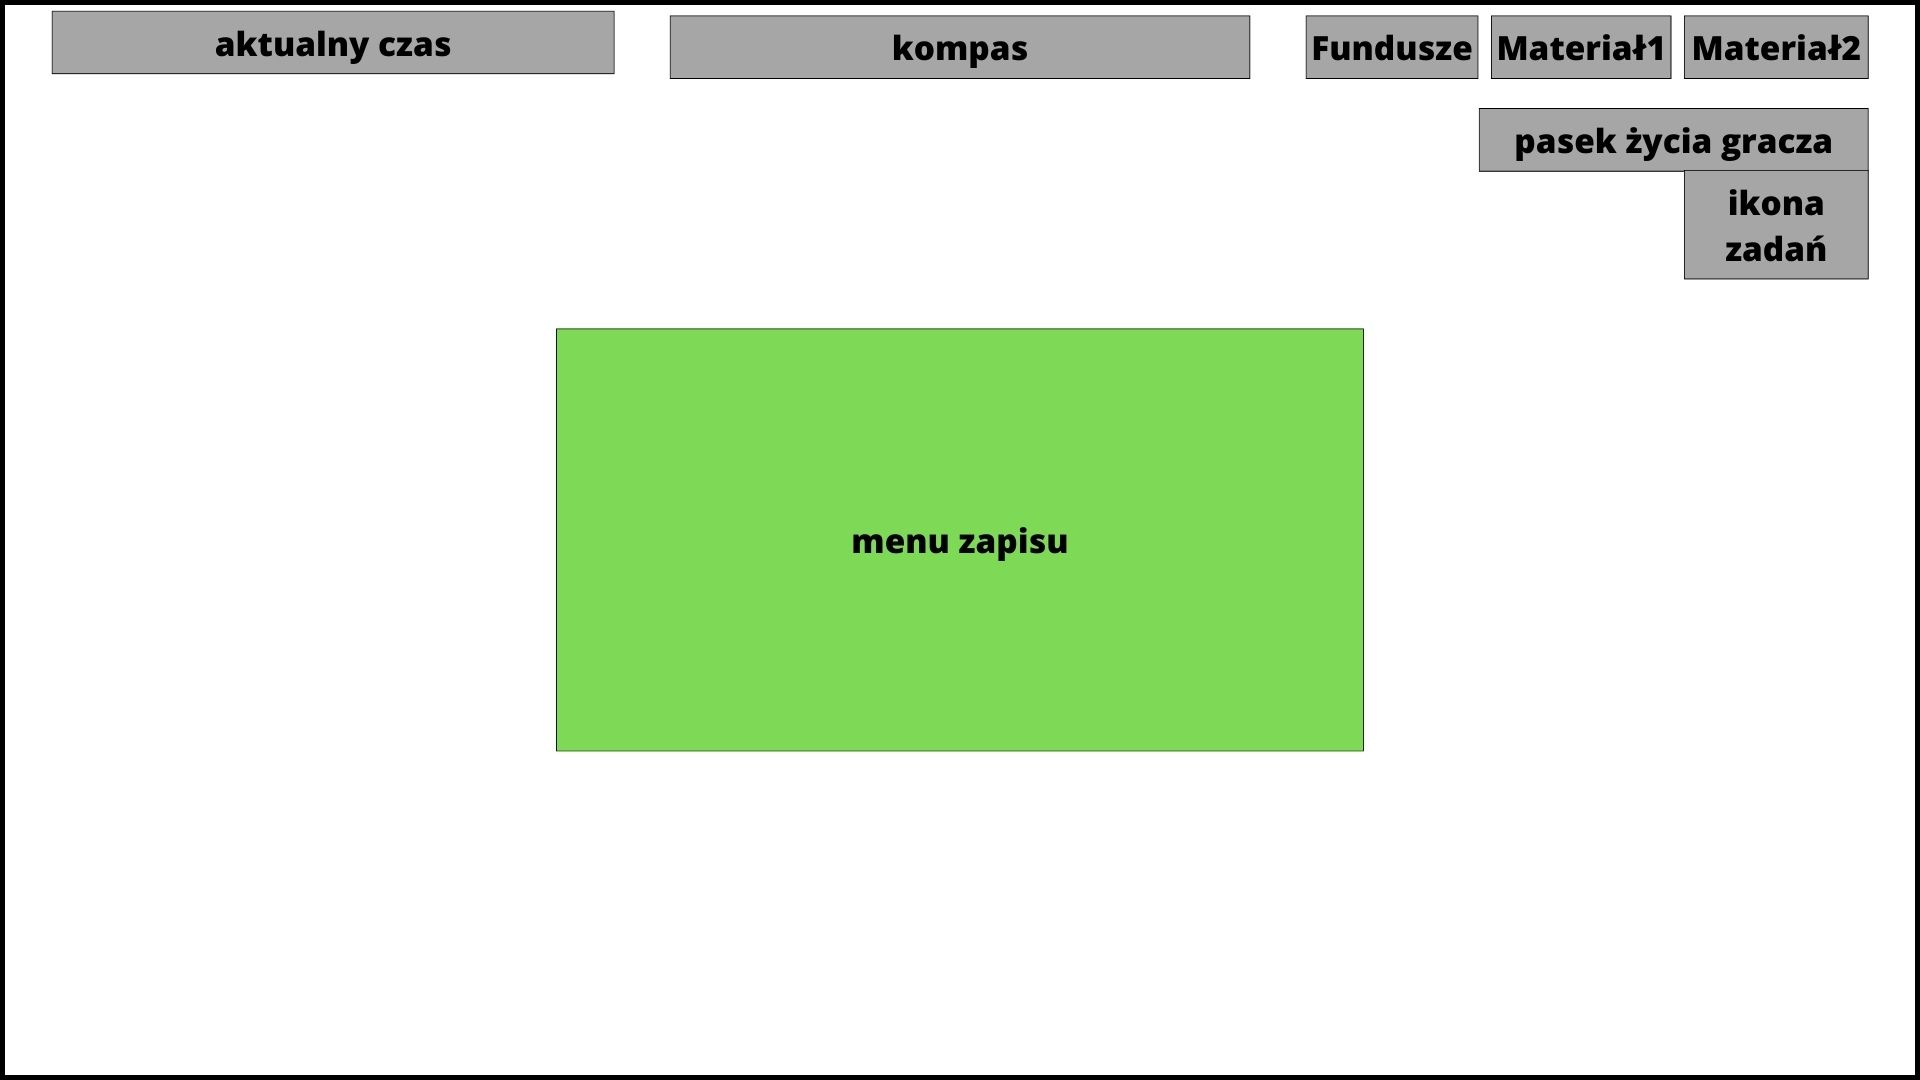
\includegraphics[width=0.9\textwidth]{images/ui/ui_proj_zapis.jpg}
    \caption{Projekt menu zapisu.}\label{fig:men_zap}
\end{figure}

\subsection{Informacja o możliwej interakcji}
W programie przewidziane są postacie i przedmioty interaktywne. Aby 
    \begin{figure}[htbp]
    \centering
    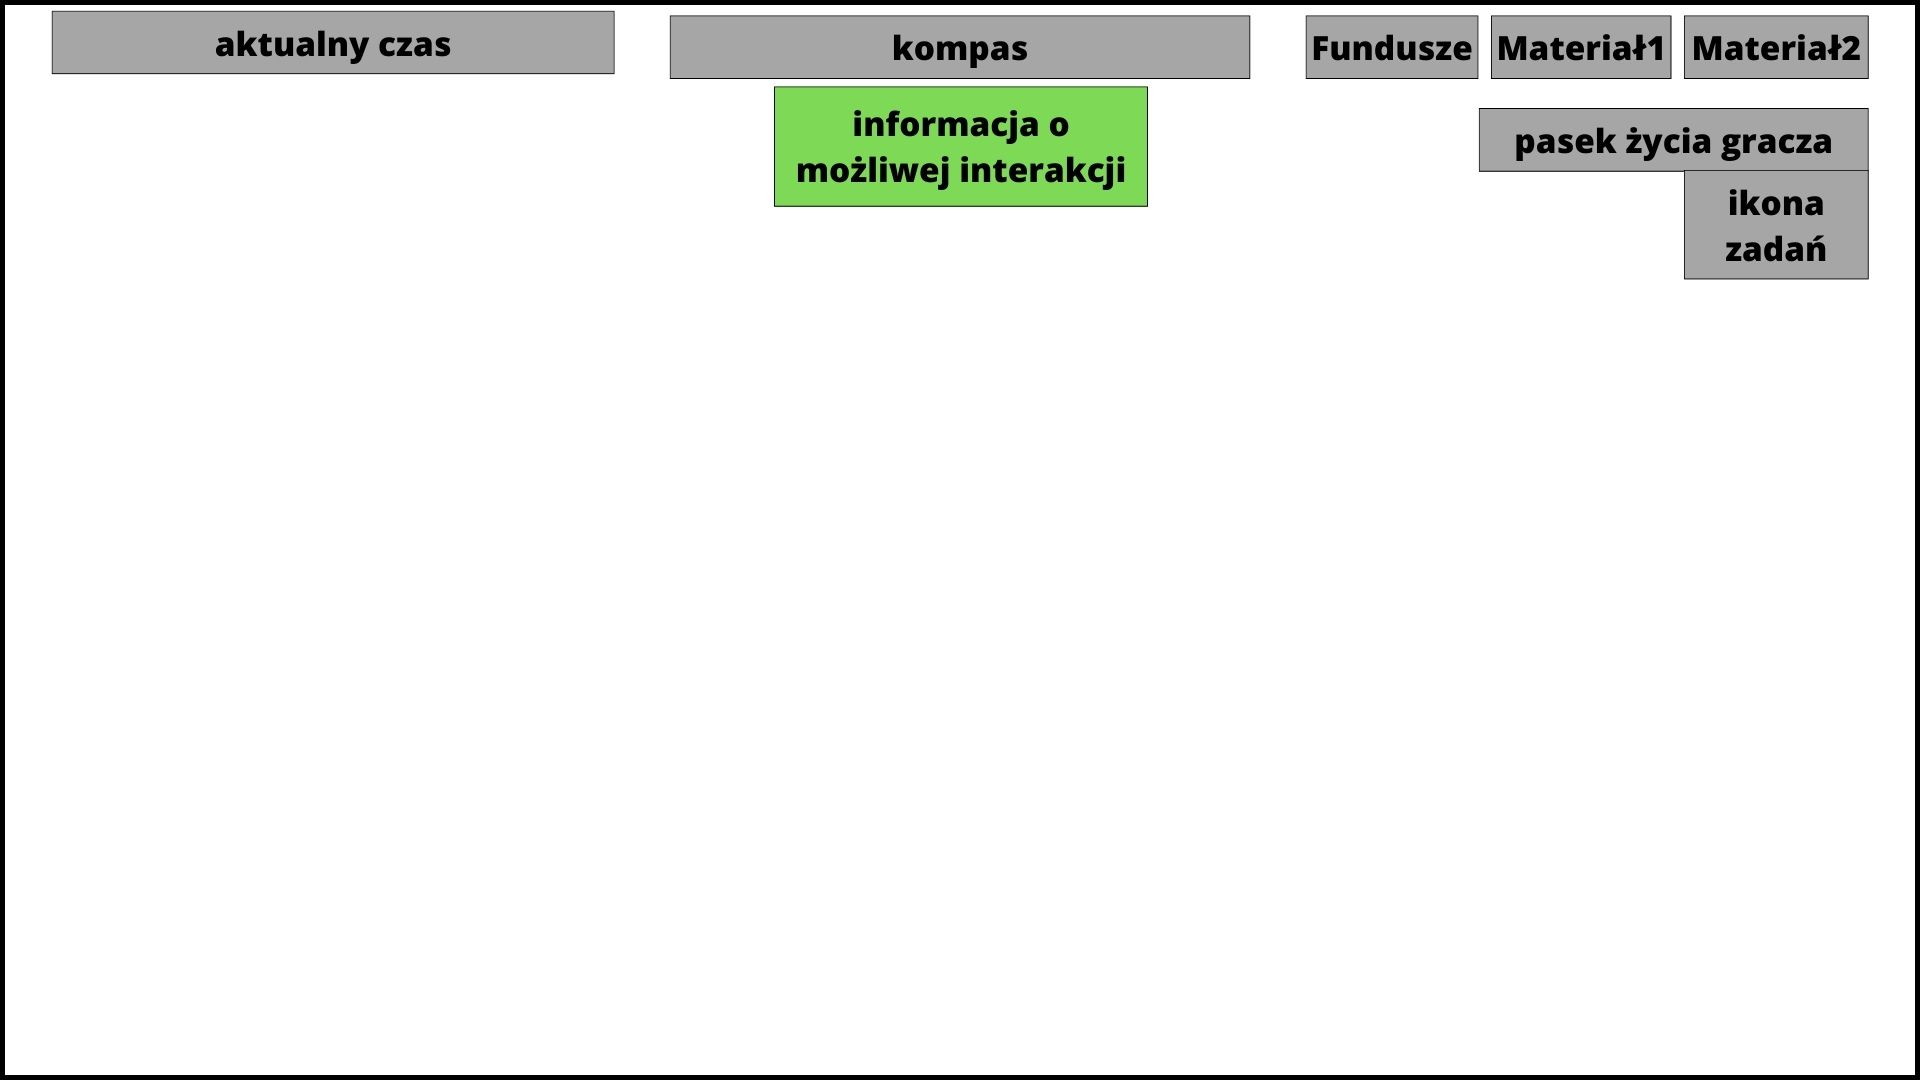
\includegraphics[width=0.9\textwidth]{images/ui/ui_prooj_interakcja.jpg}
    \caption{Projekt grafiki informującej o możliwym zaczęciu rozmowy.}\label{fig:rozmow}
\end{figure}

\subsection{Dziennik z zadaniami}

\begin{figure}[htbp]
    \centering
    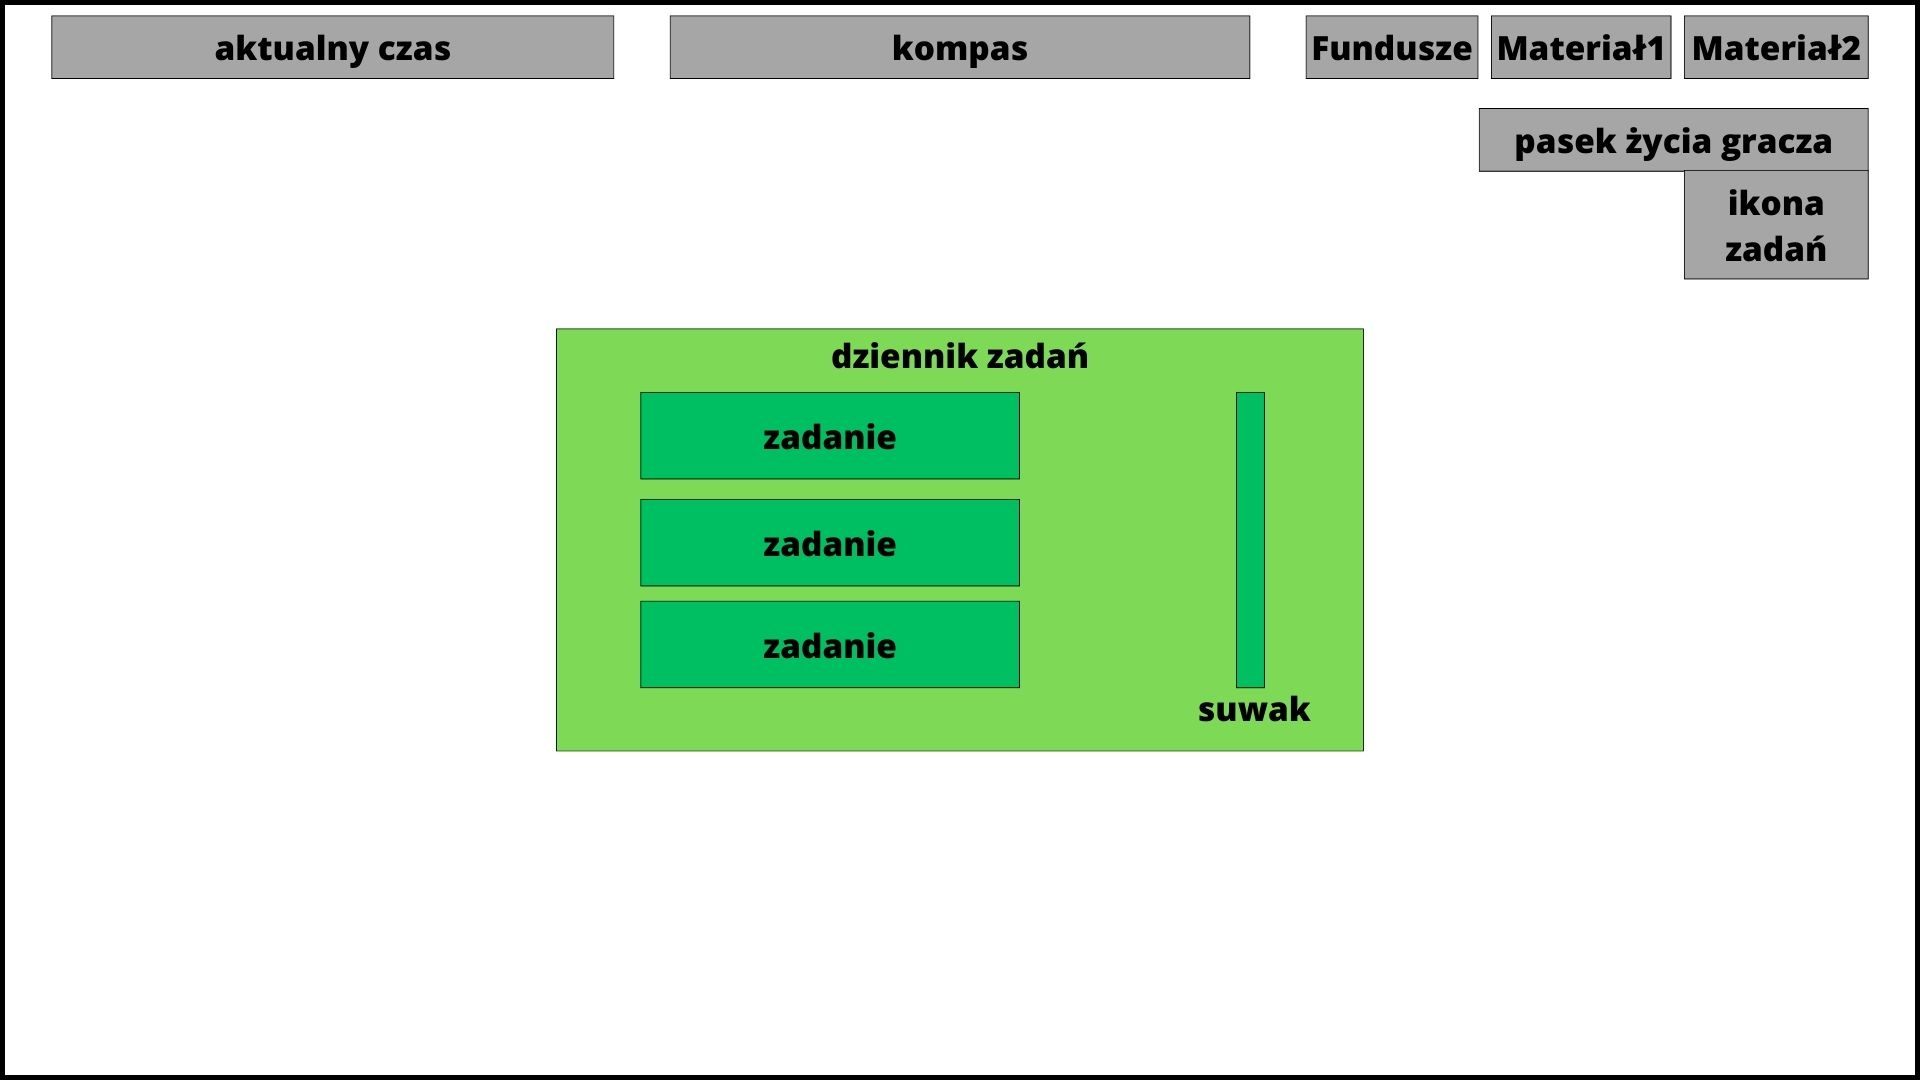
\includegraphics[width=0.9\textwidth]{images/ui/ui_proj_dziennik_zadan.jpg}
    \caption{Projekt dziennika z aktualnie zaczętym i nieukończonym zadaniem.}\label{fig:end_sc}
\end{figure}

\subsection{Ekran końca gry}

\begin{figure}[htbp]
    \centering
    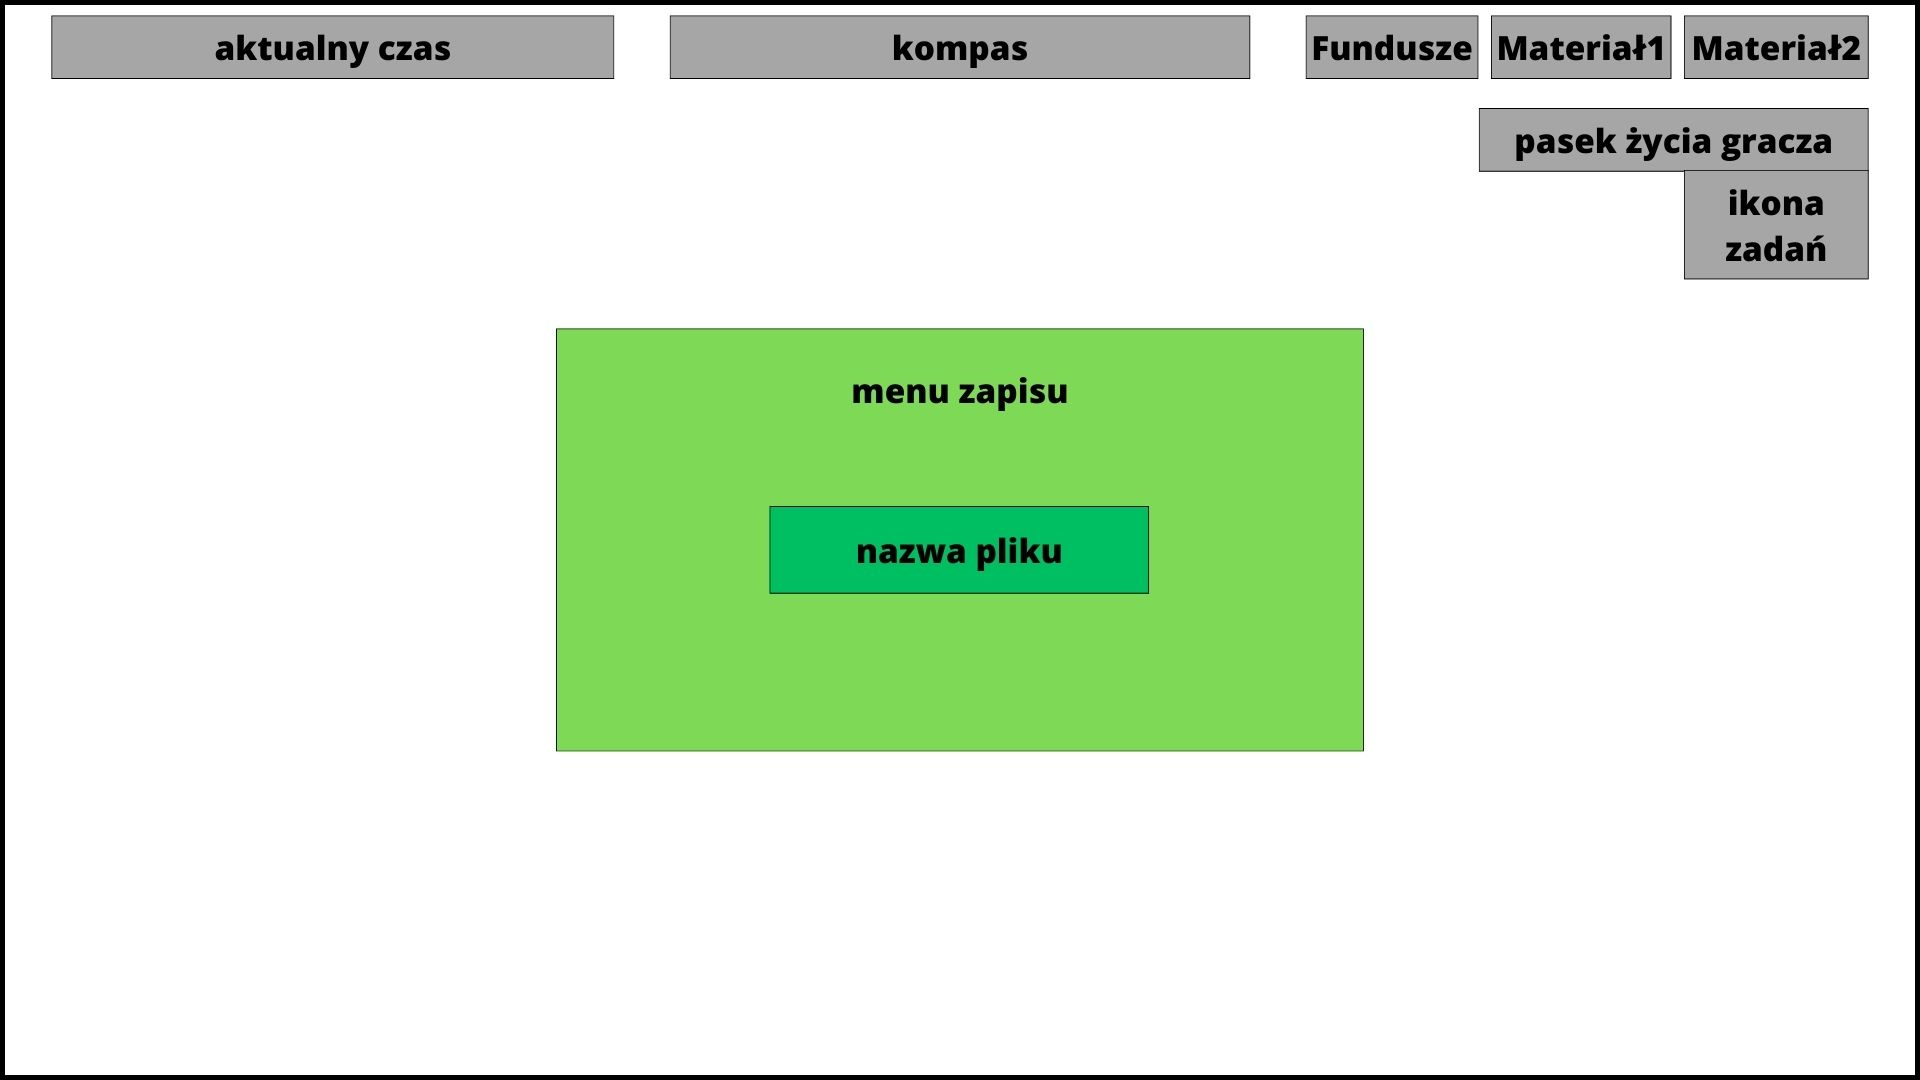
\includegraphics[width=0.9\textwidth]{images/ui/ui_prooj_koniec_gry.jpg}
    \caption{Projekt menu zapisu.}\label{fig:end_sc}
\end{figure}
